\comment{

SAM comments

I'd remove the style of addressing the reader as "you" for the thesis.

(And the "try saying that ten times fast" in 4.4.8)

In Fig4.1, say in the caption what the dashed lines on the right mean.

in 4.3.1, be more clear right at the beginning that there are two
flavours: splitting or bounding. the way it reads now, we are at first
led to think that each kd tree has two kinds of nodes.

pcode 4.3: min(p) and max(p) are ambiguous; perhaps just a comment
above that line:
# min(p) takes the minimum along every dimension
similarly, in chose_split_dimension, max(points)/min(points) should
have a comment:

A very useful optimization is to "decorate" the distance function with
an upper bound:
distance(p,q, bound=None) (see below). This tells the distance fn that
we don't care
about values >=bound. Then in 4.6, the call d = distance(p,q) can
become d = distance(p,q,closest_so_far)
and in 4.7, d = distance(p,q,range)

in 4,3,6, can you give a citation for the KDE algorithm which refines
upper&lower bounds?

4.4.9, can you provide a tiny bit of detail for the O(1) trick that
comes out of chosing the rounding wisely?

4.4.13, should you start a new subsection at the paragraph "By using
the tricks in this section..."?

4.6 point to the code location on the web

function distance(p,q, bound=None)
# return the distance between points p and q,
# if bound is passed, return values >= bound may be inaccurate
  dist_squared = 0
  if bound:
    bound_squared = bound*bound
  else:
    bound_squared = Infinity
  for dim in xrange(len(p)):
    if dist_squared >= bound_squared:
       break
   delta_dim = p[dim] - q[dim]
   dist_squared += delta_dim * delta*dim
  return sqrt(dist_squared)

}



\comment{

HOGG comments

Section 2+3, general:  I like the fact that the tricks and tips and
parts are all individually numbered, but it is also distracting to
have so many full-break headings.  What about formatting the
subsections the way LaTeX usually formats \paragraph{} so that "2.1
Data structures:" appears at the beginning of the line that currently
starts "Figure 2 shows pseudocode...".

Subsection 2.2: You don't specify when or how you change the splitting
dimension d.  Even though it *does* say in the pseudocode, I think you
should be explicit here in the text, and maybe also give some
alternatives that are also sensible.  That is, give the default method
but explain where a sensible person might make a different choice and
why.

Figure 1:  You don't explain the meaning of the dashed lines in the
caption.  Also are you really going to have red color in your thesis
here?  Also, the dashed lines are not very clear given the choppy
data; I would suggest grey or red solid lines.

Figure 3 (and subsection 2.2):  I think you should note in the
pseudocode comments and the text that traditionally you stop when the
node size goes below some threshold, but that in Section 3 you are
going to suggest an alternative.

Figure 8:  I prefer solid grey to dotted lines.

Subsection 2.6:  Either cite or explain the approximate kernel density
estimation algorithm, or both.

Section 3:   First line:  "most" or "many"?  I think you should spend
a bit more time here noting that your advice is only for the case in
which the kd-tree is edited or constructed FAR LESS FREQUENTLY than it
is searched.

Subsection 3.2:  Could you give the reader some idea of *when* you
might choose *not* to split at the median?

Subsection 3.6: I would be even a bit more explicit here, that the
data dimensions in the tree are usually only some small part of your
data, and that you have all this other information for each data point
elsewhere.  You call these "labels" in the text, but it could be all
the other columns in an enormous data base.

Section 4, para starting "We chose a very simple...": Isn't it a HUGE
DEAL that you can make bigger trees?  If so, this should be trumpeted
a bit more, here and in the abstract.  So you beat all the standard
implementations on data-set applicability alone!

Section 4, near the end of the section:  Once again, mention the
capability of making much bigger trees.

Section 5:  Give the location for the libkd download.  Perhaps it
should go to sourceforge or code.google.com, and not just
astrometry.net?  Or is it already *in* some such location?

one more thing:  I think it would be useful to indicate, among the
speed-up and optimization hints, which depend most strongly on the
data being *static* and which do not; in general, if it isn't clear,
it is worth saying what tips and tricks depend on what assumptions.
}


\newcommand{\kdtreebboxfig}{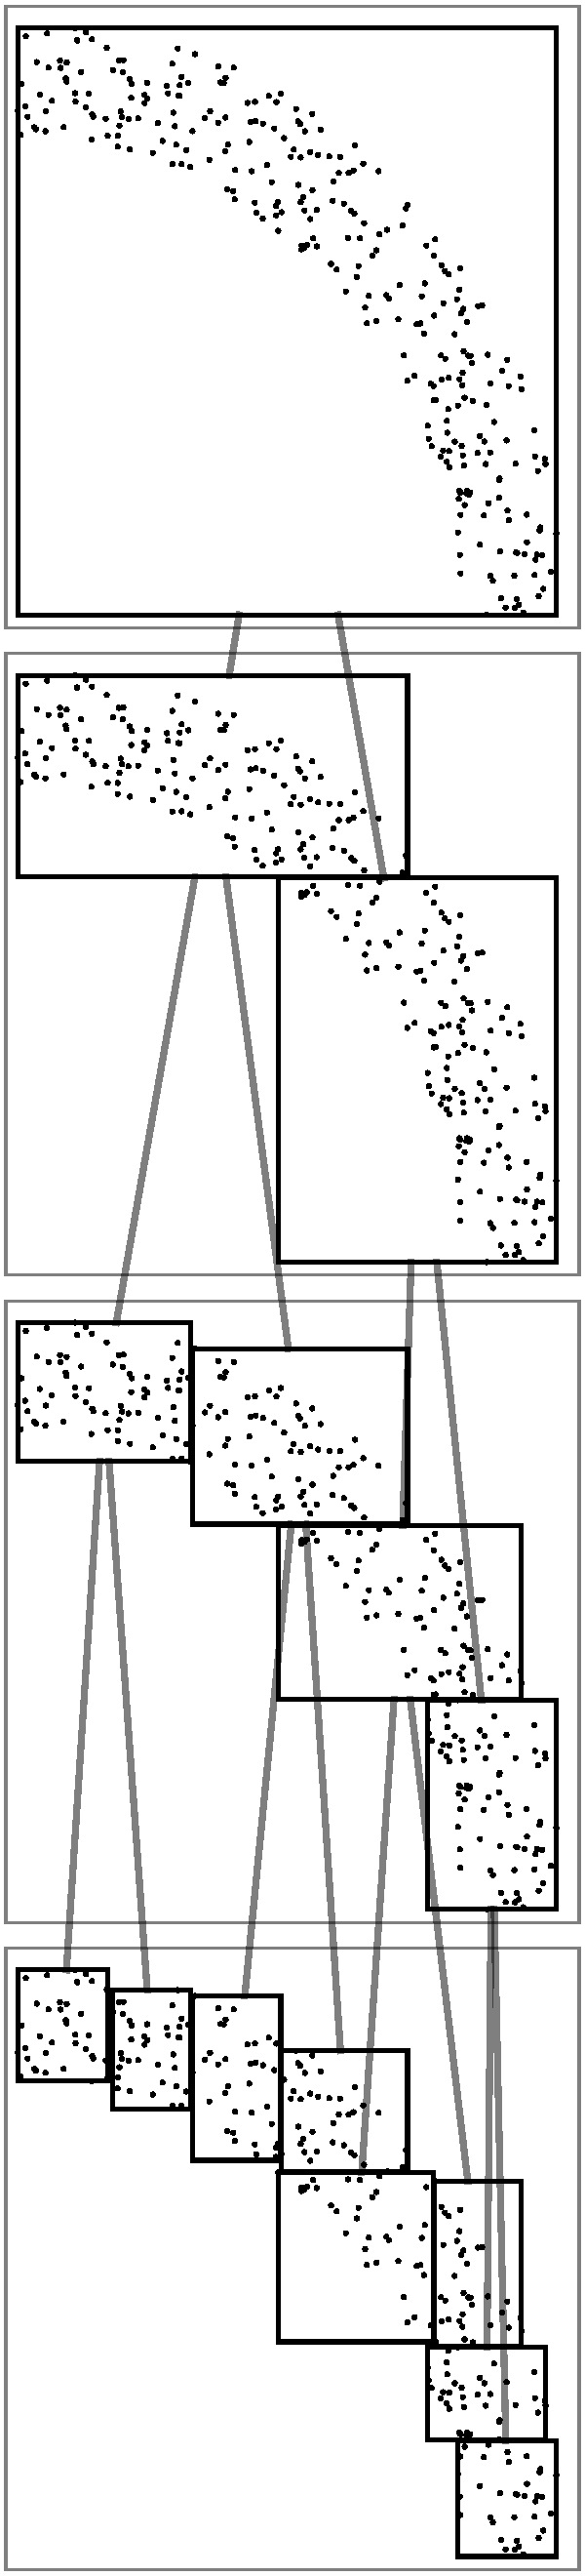
\includegraphics[width=1.000000\figunit]{kdtree-bbox}}
\newcommand{\kdtreesplitfig}{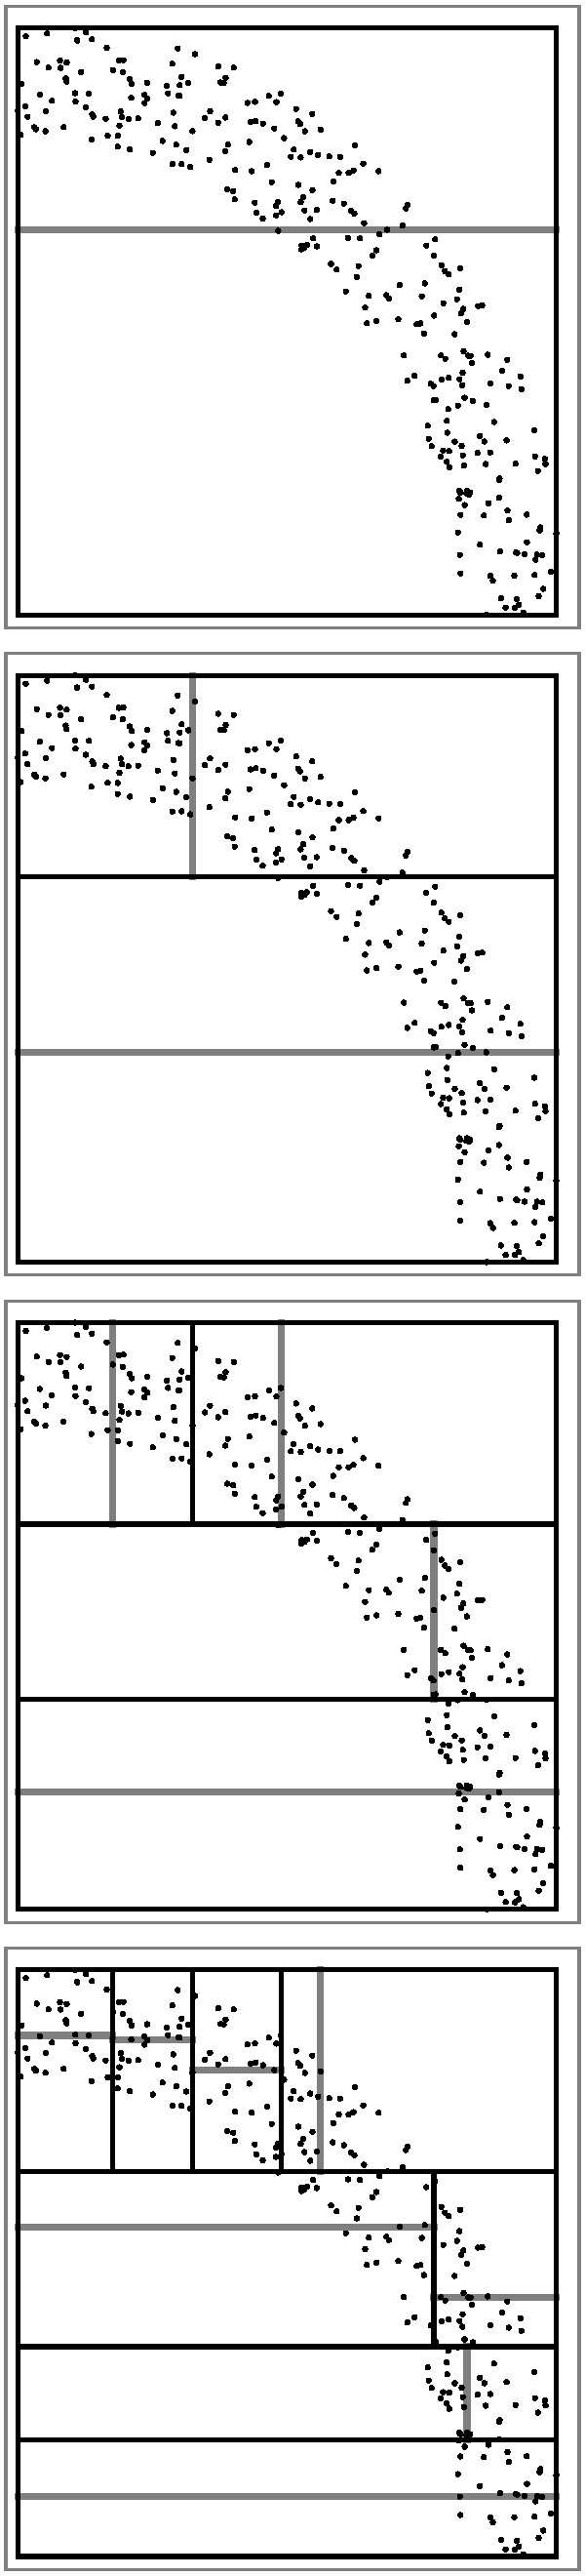
\includegraphics[width=1.000000\figunit]{kdtree-split}}
\newcommand{\mindistbboxfig}{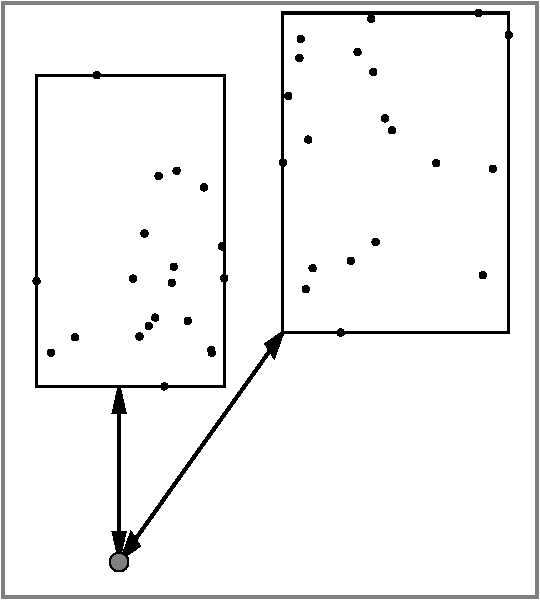
\includegraphics[width=0.900000\figunit]{mindist-bbox}}
\newcommand{\mindistsplitfig}{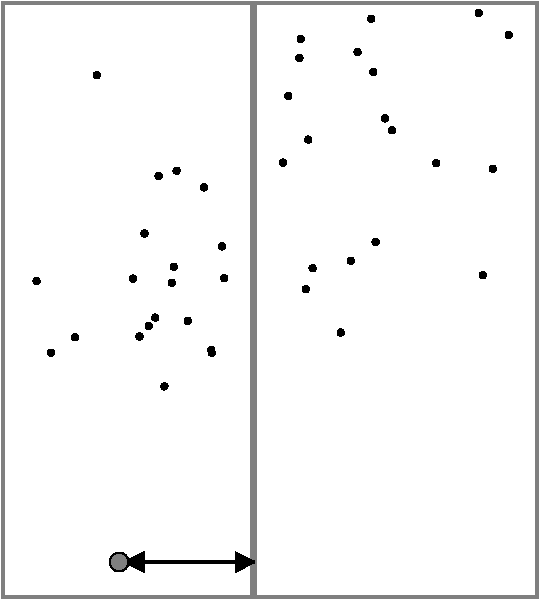
\includegraphics[width=0.900000\figunit]{mindist-split}}
%% see   getbb.sh  to find the bounding-box of the ink in a figure.

%% The sizes shown are from getbb.sh using 12pt font in figures.

%% pgf/tikz often believes that the bounding-box extends beyond the
%% extent of the ink, so forcing it to the ink size doesn't always
%% work (the figure overflows onto page 2)

% 169 x 65
\newcommand{\pointerlessfigwidth}{170pt}
\newcommand{\pointerlessfigheight}{76pt}

% 267 x 249
\newcommand{\permutefigwidth}{268pt}
\newcommand{\permutefigheight}{249pt}

% 251 x 162
\newcommand{\applypermfigwidth}{252pt}
\newcommand{\applypermfigheight}{162pt}

% 263 x 119
\newcommand{\ronlyfigwidth}{268pt}
\newcommand{\ronlyfigheight}{122pt}

% 233 x 93
\newcommand{\transposefigwidth}{234pt}
\newcommand{\transposefigheight}{93pt}

% 145 x 58
\newcommand{\bitpackfigwidth}{149pt}
\newcommand{\bitpackfigheight}{66pt}

\newcommand{\kdbarmemfig}{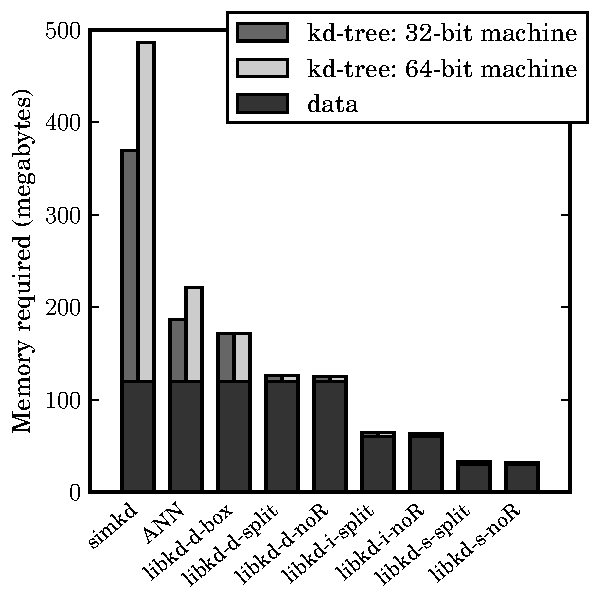
\includegraphics[width=1.000000\figunit]{kd-bar-mem}}
\newcommand{\kdbarspeedfig}{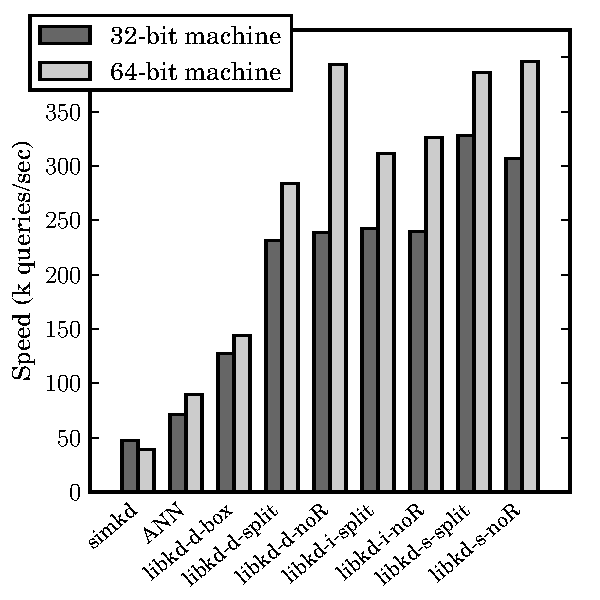
\includegraphics[width=1.000000\figunit]{kd-bar-speed}}


\section{Introduction}

  The \kdtree is a simple yet versatile data structure for speeding up
  searches in $k$-dimensional data sets.  It applies to
  nearest-neighbour queries, which arise in many computer vision
  applications such as vector quantization and template matching.  It
  also applies to a family of related problems such as range search
  (finding all points within a given radius of a query), $K$-nearest
  neighbours, and approximate kernel density estimation.  Over its
  long history the \kdtree has accumulated many extensions and
  variations making the literature difficult to comprehend.
  This \doctype presents a modern view of the \kdtree.  It also points
  out a number of optimizations that can increase the performance by
  an order of magnitude over existing publicly available
  implementations while also reducing the memory requirements---or
  increasing the size of the largest \kdtree that be constructed in a given
  amount of memory.

\section{The standard \kdtree}


\Kdtrees have accelerated spatial queries for over thirty years.
\Kdtrees speed up N-body simulations, search, object recognition,
ray tracing, template matching, kernel density estimation, and more.
%But what \emph{is} a \kdtree?



Imagine you have a classification problem.  You have a million
labelled 2-dimensional data points (``feature vectors'') in the unit
square.  You also have a set of a million unlabelled data points, and
a deadline.  You decide to run nearest-neighbour classification.
After a moment of thought you realize that if you compare every
labelled feature to every unlabelled feature you will have to do
$10^{12}$ comparisons.  Your deadline looms.  Upon further reflection,
you decide to split the labelled points in half: the ones with $x \le
\half$ and the ones with $x > \half$.  When you want to
find the nearest neighbour of an unlabelled point that has $x \le
\half$, you look in the first set of labelled points.  Most of
the time, you find that the distance between the unlabelled point and its
nearest labelled neighbour is less than the distance to the $x =
\half$ boundary.  You don't even need to look at the second set
of labelled points!

\begin{figure}
\begin{center}
\begin{tabular}{@{}c@{\hspace{5em}}c@{}}
 % as big as they can be before overflowing the page...
 % created by kdtree-tests/tree-figs.py
 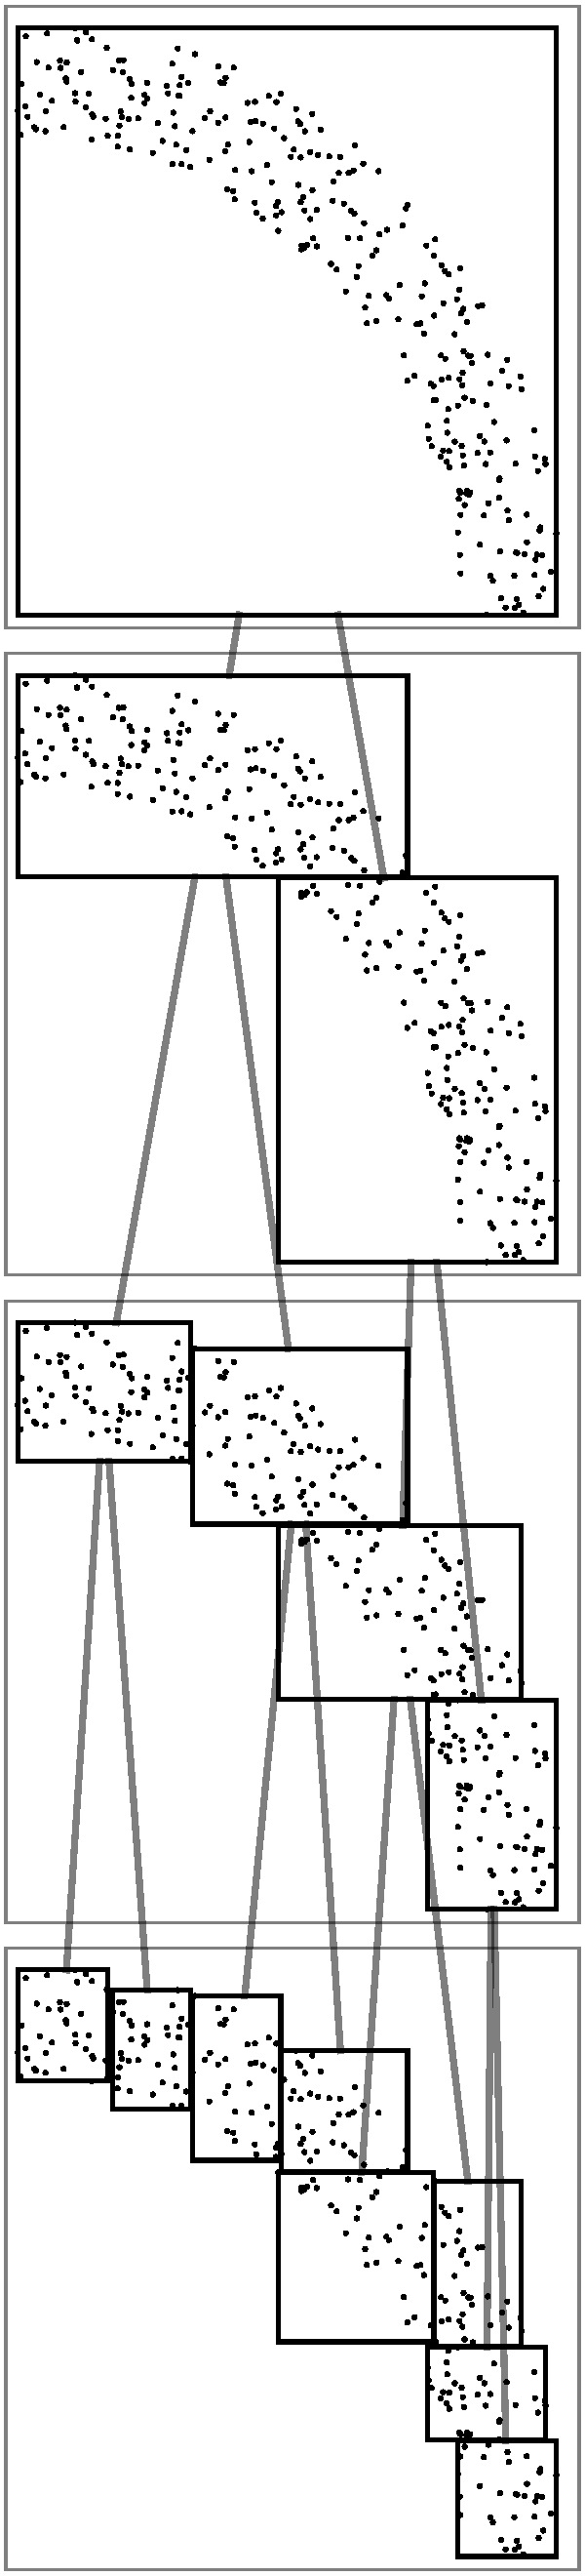
\includegraphics[height=0.82\textheight]{kdtree-bbox}&
 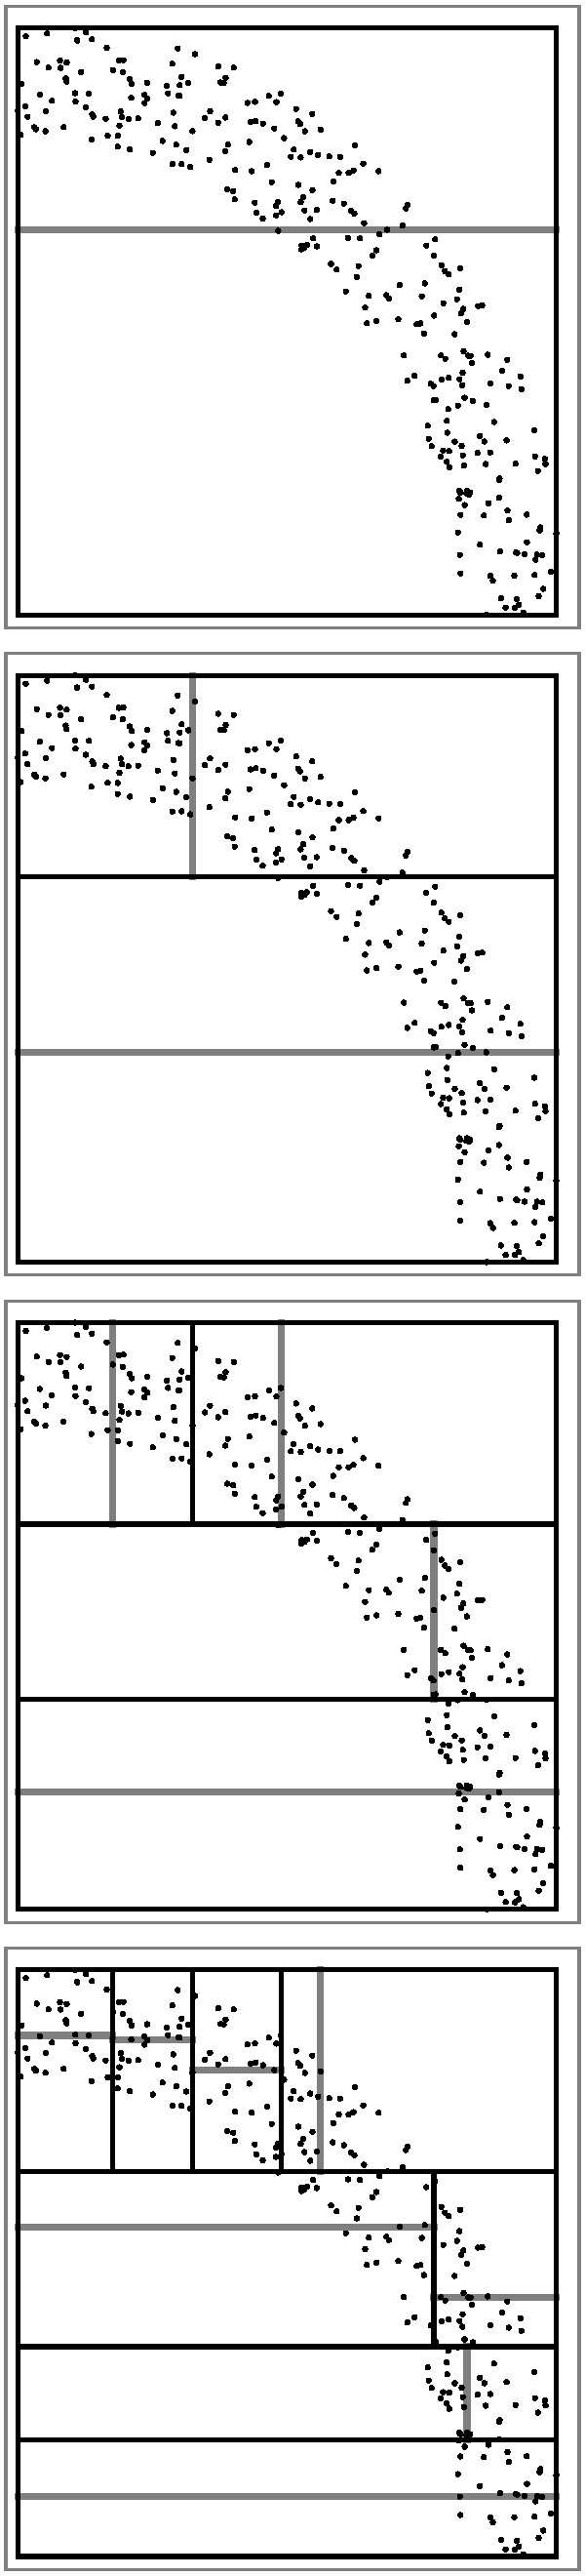
\includegraphics[height=0.82\textheight]{kdtree-split}%
\end{tabular}
\end{center}
\caption{Two varieties of \kdtree.  \captionpart{Left:} A \kdtree with bounding boxes.
Parent-child relationships are shown by gray lines.
\captionpart{Right:} A \kdtree with splitting planes.  The splitting plane at each
node is shown by a gray line.  The top box is the root node.
Parent-child relationships are not shown in order to avoid cluttering
the figure.}
\label{fig:tree}
\end{figure}




While waiting for your algorithm to finish, you \mbox{remember}
recursion.  You decide to split the labelled points in half again.
{\small And again.}  {\scriptsize And again.}  {\tiny And again.}  You
just invented \kdtrees.  If it was 1975 you would be the first, and
win a prize \cite{bentley1975}.


You used a \kdtree to speed up nearest neighbour search (find the
closest data point to the query point).  They are also useful for
\emph{range search} (find all data points within some radius of a
query point) and more complex queries such as \emph{approximate kernel
density estimation}.



A \kdtree is a type of \emph{Binary Space Partition} tree.  Each node
in the tree represents a portion of space.  In \kdtrees the portion of
space is an axis-aligned bounding box.%
\footnote{In the example above, the first node you created had the
bounding box $x \in [0, \half]$ and $y \in [0, 1]$.}  Each node has
two children which split the node's space in two.  This split is
usually chosen so that half the data points go into each child.  A
node's axis-aligned bounding box is either explicitly stored, or
implicitly defined by its ancestors' splitting planes.


% binary, balanced and complete.


%Related stuff.
%\cite{friedman1977, sproull1991}
%Competition: \cite{arya1998}, \cite{uhlmann1991}, \cite{moore2000},
%\cite{datar2004}; \cite{hjaltason2003} (survey).

\Kdtrees work well in low-dimensional spaces (opinions vary, but say up to 15).
In high dimensions, other data structures may work better \cite{bohm2001}.

\def\ignore#1{}
\ignore{}{Below, we first describe the core structure of \kdtrees, but note that the foundational implementation is not the most efficient. We then move to the comprehensive series of implementation ``tricks'' that must be considered for optimal performance. Finally, we compare our implementation, {\tt libkd} (incorporating the efficiencies described), with two previously released \kdtree implementations: {\tt ANN} \cite{arya1998} and {\tt Simple \kdtrees} \cite{simkd} (abbreviated to {\tt simkd}) to show the considerable level of speed-ups that can be attained.}

\section{\Kdtree implementation}

\subsection{Data structures}
\label{sec:datastruct}

\Figref{code:datastruct} shows pseudocode for \kdtree data
structures.  There are two types of \kdtree nodes listed, {\tt
SplittingNode} and {\tt BoundingBoxNode}.  In this \doctype, a \kdtree
contains nodes of only one type, but of course it is possible to store
both the splitting plane and bounding box of each node if required by
the application.  {\tt BoundingBoxNode}s contain two points which
define the maximum and minimum corners of the bounding box.  {\tt
SplittingNode}s do not contain an explicit representation of their
spatial extent.  Instead, each node contains a split dimension and
position.  A {\tt SplittingNode}'s bounding box is implicitly
described by the splits of its ancestors.


The two representations have different performance characteristics on
different data distributions.  For example, the benchmark in
\secref{sec:speed} favours splitting planes.  Structured data sets
where the dimensions are correlated and the data point distribution is
clumpy work well with bounding box nodes.


Please note that these data structures are only for explaining the
\kdtree; for practical implementation details see
\secref{sec:impl}.



\subsection{Construction}


\Kdtree construction starts with a set of points.  Construction begins by
creating a root node which contains all of the data points.  The root
node is split into two halves by choosing a splitting dimension
(usually the dimension with the largest spread) and a splitting
position (usually the median value of the points along that
dimension).  Then, the set of points whose position along the
splitting dimension is less than the splitting position are put in the
left child.  The remaining points are put in the right child.
Construction proceeds recursively until the nodes at the lowest level
of the tree contain some small number of points (perhaps 10).  See
\figref{code:build} for pseudocode.

\clearpage

\begin{figure}
  \begin{pcode}
      \class KDTree: \\
      \> Node root \\
      \\
      \class Node: \\
      \> \codecomment{empty superclass for leaf and internal nodes} \\
      \\
      \class InternalNode extends Node: \\
      \> \codecomment{superclass of bounding box} \\
      \> \codecomment{and splitting plane nodes} \\
      \> Node left\_child \\
      \> Node right\_child \\
      \\
      \class BoundingBoxNode extends InternalNode: \\
      \> \codecomment{lower and upper corners of the bounding box} \\
      \> point lower \\
      \> point upper \\
      \\
      \class SplittingNode extends InternalNode: \\
      \> \codecomment{splitting plane dimension and value} \\
      \> int  split\_dimension \\
      \> real split\_position \\
      \\
      \class LeafNode extends Node: \\
      \> point[] points\_owned
  \end{pcode}
  \caption{Data structures for \kdtree nodes.
    Each {\tt LeafNode} contains a set of $D$-dimensional {\tt point}s.
    All nodes in a \kdtree are either of type {\tt BoundingBoxNode} or
    {\tt SplittingNode}.
    In practice, more efficient structures should be used; see \secref{sec:impl}.}
  \label{code:datastruct}
\end{figure}

\begin{figure}
\begin{pcode}
  \func build\_kdtree(point[] p, int nleaf, bool b\_boxes): \\
  \> t = new KDTree() \\
  \> t.root = build\_node(p, nleaf, b\_boxes) \\
  \> return t \\
  \\
  \codecomment{Build a \kdtree node from a set of points.} \\
  \func build\_node(point[] p, int nleaf, bool boxes): \\
  \> \codecomment{if the set of points is small enough...} \\
  \> if p.size() <= nleaf: \\
  \>\> \codecomment{create a leaf node.} \\
  \>\> return new LeafNode(p) \\
  \> \codecomment{else, choose a splitting dimension...} \\
  \> split\_dim = choose\_split\_dimension(p) \\
  \> \codecomment{and split the points along that dimension.} \\
  \> (p\_left, p\_right, split\_pos) = partition(p, split\_dim) \\
  \> if boxes: \\
  \>\> n = new BoundingBoxNode() \\
  \>\> n.lower = min(p) \\
  \>\> n.upper = max(p) \\
  \> else: \\
  \>\> n = new SplittingNode() \\
  \>\> n.split\_dimension = split\_dim \\
  \>\>  n.split\_position = split\_pos \\
  \> \codecomment{recurse on the two point sets} \\
  \> \codecomment{to create the child nodes.} \\
  \> n.left\_child \spc = build\_node(p\_left, \spc nleaf, boxes) \\
  \> n.right\_child = build\_node(p\_right, nleaf, boxes) \\
  \> return n \\
  \\
  \codecomment{Typical: split the dimension with largest range.} \\
  \func choose\_split\_dimension(points): \\
  \> return argmax(max(points) - min(points)) \\
  \\
  \codecomment{Typical: split at the median value.} \\ % to yield a balanced tree.} \\
  \func partition(points, dim): \\
  \> \codecomment{find the median value in the splitting dimension} \\
  \> split\_val = median(points, dim) \\
  \> \codecomment{grab points on each side of the partition.} \\
  \> p\_left  \spc = [p in points
              where p[dim] <= split\_val] \\
  \> p\_right = [p in points
              where p[dim] > \spc split\_val] \\
  \> return (p\_left, p\_right, split\_val)
\end{pcode}
\caption{Pseudocode for \kdtree construction.}
\label{code:build}
\end{figure}



\subsection{Distance bounds}

Fundamentally, \kdtree algorithms are about pruning nodes that don't need
to be examined.  The primary tool to achieve this is the \mindist
function, which provides a lower bound on the distance between a point and
any point that lives in the region owned by a node.
Intuitively, this is the distance from a point to the closest corner or closest
edge of the node.

The form of the \mindist function depends on the representation of a \kdtree
node.  For \kdtrees that have bounding boxes, one computes the
\mindist to an individual node.  For \kdtrees that only store the splitting plane,
it makes more sense to compute the \mindist to each of the node's two children.
An illustration is given in \figref{fig:mindist} and pseudocode in
\figref{code:mindist}.


\begin{figure}
\begin{center}%
\begin{tabular}{@{}c@{\hspace{3em}}c@{}}
\mindistbboxfig &
\mindistsplitfig
\end{tabular}
\end{center}
\caption{\captionpart{Left:} \mindist for a \kdtree node with bounding boxes.
The query point is shown as a gray dot, and the \mindist s to the two
boundig-boxes are shown by the arrows.
\captionpart{Right:} \mindist for a \kdtree node with only the splitting
dimension and value.  The \mindist is zero for the child on the same
side of the splitting plane as the query point; for the other child
the \mindist is simply the distance in the splitting dimension from
the query to the splitting plane.}
\label{fig:mindist}
\end{figure}

\begin{figure}
\begin{pcode}
\func mindist\_to\_box(point p, BoundingBoxNode n): \\
\>   mindist = 0 \\
\>   for each dimension d: \\
\>\>      if p[d] > n.upper[d]: \\
\>\>\> \codecomment{p is above the bounding} \\
\>\>\> \codecomment{box in this dimension} \\
%\>\>\> \codecomment{p is above the bounding box in this dimension} \\
\>\>\>         diff = n.upper[d] - p[d] \\
\>\>      else if p[d] < n.lower[d]: \\
\>\>\> \codecomment{p is below the bounding} \\
\>\>\> \codecomment{box in this dimension} \\
\>\>\> diff = p[d] - n.lower[d] \\
\>\>      else: \\
\>\>\> \codecomment{p is within the bounding} \\
\>\>\> \codecomment{box in this dimension} \\
%\>\>\> \codecomment{p is within the bounding box in this dimension} \\
\>\>\>      diff = 0 \\
\> mindist += diff * diff \\
\> return sqrt(mindist) \\
\\
\func mindist\_to\_left\_child(point p, SplittingNode n): \\
\>   d = n.split\_dimension \\
\>   if p[d] > n.split\_position: \\
\>\>   \codecomment{point is on the right side} \\
\>\>   \codecomment{of node's splitting plane} \\
%\>\>   \codecomment{point is on the right side of node's splitting plane} \\
\>\>      return p[d] - n.split\_position \\
\>   return 0 \\
\\
\func mindist\_to\_right\_child(point p, SplittingNode n): \\
\>   d = n.split\_dimension \\
\>   if p[d] < n.split\_position: \\
\>\>   \codecomment{point is on the left side} \\
\>\>   \codecomment{of node's splitting plane.} \\
%\>\>   \codecomment{point is on the left side of node's splitting plane.} \\
\>\>      return n.split\_position - p[d] \\
\>   return 0
\end{pcode}
\caption{Pseudocode for \mindist.  \captionpart{Top:} for \kdtrees with bounding boxes.
\captionpart{Bottom:} for \kdtrees with splitting
planes.}
\label{code:mindist}
\end{figure}

\subsection{Nearest neighbour}

Given a set of data points and a query point, solving the nearest neighbour
problem consists of finding the data point that is closest to the query.
Specifically, given query point $\mathbf{q}$, find
\begin{equation}
\mathbf{x}_{\mathit NN} = \argmin_{i} \| \mathbf{x}_i - \mathbf{q} \|_{2} \quad .
\end{equation}
The algorithm is of the \emph{branch and bound} variety
\cite{land1960}: the tree is traversed, maintaining a \emph{pruning
distance}---the distance to the nearest data point found so far.  In
addition, the set of nodes that might contain the solution are stored
in a stack or priority queue ordered by \mindist.  If a node is
encountered whose \mindist to the query point is larger than the
pruning distance, it is discarded because it cannot contain the
solution.  When a leaf node is encountered, its data points are
examined individually.  If any data point is closer than the pruning
distance, that point becomes the nearest neighbour found so far, and
the pruning distance is set to the point's distance to the query
point.  The algorithm begins by setting the pruning distance to
$+\infty$ and placing the root node on the stack.  See the pseudocode
in \figref{code:nn}.


\subsection{Rangesearch}

In the rangesearch problem, the goal is to find all points that are
within a certain radius of the query point.  Specifically, given query
point $\mathbf{q}$, radius $r$, and a set of points $\mathbb{X}$, find
the set of points
\begin{equation}
\left\{
 \ \mathbf{x}
\ \Big| \ \| \mathbf{x} - \mathbf{q} \|_{2} \le r,\ \mathbf{x}\in\mathbb{X} \
\right\}
\quad .
\end{equation}
Range search is simpler than nearest neighbour search because the
pruning distance is fixed.  This implies that the list of nodes that
must be inspected does not depend on the order of tree traversal.  At
each node the \mindist to the query point is computed.  If it is
larger than the search radius, it is pruned because it cannot possibly
contain any data points within the radius.  See the pseudocode
in \figref{code:rangesearch}.


\begin{figure}
\begin{pcode}
\codecomment{Input: root of a \kdtree, and a query point q} \\
\codecomment{Output: (x, distance(x, q)) such that x is the} \\
\codecomment{  nearest neighbour of q in the \kdtree} \\
%\codecomment{  x = argmin dist(x, q) for all x in the \kdtree} \\
\func nearest\_neighbour(KDTree t, point q): \\
%1234567890123456789012\=\kill
%\> real pruning\_distance=+inf): \\
%\tabstops
\>   nodestack.push(t.root) \\
\>   closest\_so\_far = +inf \\
\>   nearest\_neighbour = null \\
\>   while nodestack is not empty: \\
\>\>      n = nodestack.pop() \\
\>\>      if mindist(n, q) >= closest\_so\_far: \\
\>\>\>         \codecomment{this node can be pruned.} \\
\>\>\>         continue \\
\>\>      if n.is\_leaf(): \\
\>\>\>         \codecomment{leaf node: examine individual points} \\
\>\>\>         for p in n.points\_owned: \\
\>\>\>\>            d = distance(p, q) \\
\>\>\>\>            if d < closest\_so\_far: \\
\>\>\>\>\>               \codecomment{nearest neighbour found so far} \\
\>\>\>\>\>               closest\_so\_far = d \\
\>\>\>\>\>               nearest\_neighbour = p \\
\>\>      else: \\
\>\>\>         \codecomment{find the mindists to the child nodes} \\
\>\>\>         mindist\_L = mindist\_to\_left\_child(n, q) \\
\>\>\>         mindist\_R = mindist\_to\_right\_child(n, q) \\
\>\>\>         \codecomment{visit the closest child first} \\
\>\>\>         \codecomment{(by stacking the farther child first)} \\
\>\>\>         if mindist\_L > mindist\_R: \\
\>\>\>\>            nodestack.push(n.left\_child) \\
\>\>\>\>            nodestack.push(n.right\_child) \\
\>\>\>         else: \\
\>\>\>\>            nodestack.push(n.right\_child) \\
\>\>\>\>            nodestack.push(n.left\_child) \\
\>   return (nearest\_neighbour, closest\_so\_far)
\end{pcode}
\caption{Pseudocode for nearest neighbour search.  The algorithm maintains
a stack of nodes to explore and a pruning distance ({\tt
closest\_so\_far}), which is the distance to the nearest data point
found so far.  Any node whose
\mindist is greater than the pruning distance is pruned.}
\label{code:nn}
\end{figure}


%\begin{tikzpicture}[remember picture, overlay]
%  \node [xshift=0.3em, yshift=-1in] (A) at (current page.north) {};
%  \node [xshift=-0.3125in] (tl) at (A.center) {};
%  \node [yshift=-8.875in] (bl) at (tl.center) {};
%  \node [xshift=-3.28125in] (br) at (bl.center) {};
%  \node [xshift=-3.28125in] (tr) at (tl.center) {};
%  \draw [blue] (tl) -- (tr) -- (br) -- (bl) -- (tl);
%\end{tikzpicture}


\begin{figure}
\begin{pcode}
\codecomment{Input: A \kdtree, a query point q, and a range} \\
\codecomment{Output: The set [(x, distance(x, q)), ...] } \\
\codecomment{  such that distance(x, q) < range} \\
\codecomment{  for all x in the \kdtree} \\
\func range\_search(KDTree t, point q, real range): \\
\>   results = [] \codecomment{empty list} \\
\>   range\_search\_helper(t.root, q, range, results) \\
\>   return results \\
\\
\func range\_search\_helper(Node n, point q, \\
  12345678901234567890123\=\kill
  \> real range, list res): \\
  \tabstops
\>   if is\_leaf(n): \\
 \>\>     for each p in n.points\_owned: \\
\>\>\>         d = distance(p,q) \\
\>\>\>         if d < range: \\
\>\>\>\>            res.append( (p, d) ) \\
\>\>      return \\
\>   if mindist\_to\_left\_child(n, q) < range: \\
\>\>      range\_search\_helper(n.left\_child, \spc q, range, res) \\
\>   if mindist\_to\_right\_child(n, q) < range: \\
\>\>      range\_search\_helper(n.right\_child, q, range, res)
\end{pcode}
\caption{Pseudocode for range search.}
\label{code:rangesearch}
\end{figure}

%For \kdtrees that only store the splitting plane, the algorithm is slightly
%simpler.  Each time we examine a non-leaf node, we determine whether the
%query point lies to the left or right of the splitting plane.  We place the
%opposite child on the stack, followed by the child that owns the space
%containing the query point.  A lower bound on the distance from the query
%point to the opposite child is simply the distance in the splitting dimension
%of the query to the splitting plane.

% Pseudocode...


% Good seed: 1197089319

\begin{figure}
  \begin{center}
    \newlength{\nnfigw}
    \setlength{\nnfigw}{0.259\textwidth}
	\newlength{\nnspc}
    \setlength{\nnspc}{6pt}
	  \begin{tabular}{@{}c@{\hspace{\nnspc}}c@{\hspace{\nnspc}}c@{}}
  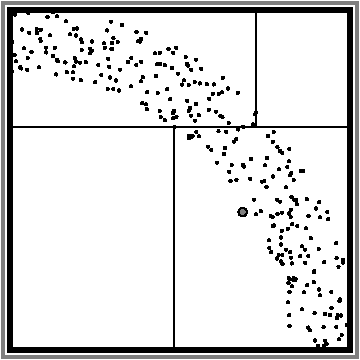
\includegraphics[width=\nnfigw]{nn-bbox-1} &
  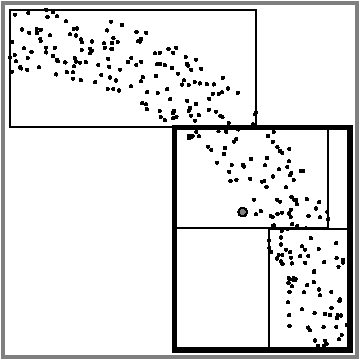
\includegraphics[width=\nnfigw]{nn-bbox-2} &
  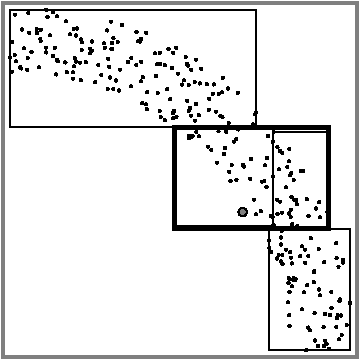
\includegraphics[width=\nnfigw]{nn-bbox-3} \\
  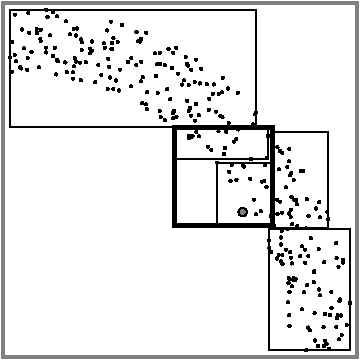
\includegraphics[width=\nnfigw]{nn-bbox-4} &
  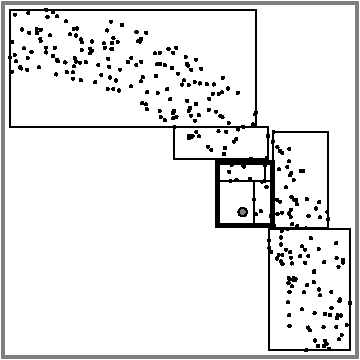
\includegraphics[width=\nnfigw]{nn-bbox-5} &
  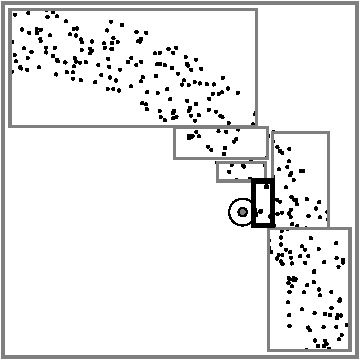
\includegraphics[width=\nnfigw]{nn-bbox-6}
  \end{tabular}

  \vspace{20pt}

  \begin{tabular}{@{}c@{\hspace{\nnspc}}c@{\hspace{\nnspc}}c@{}}
      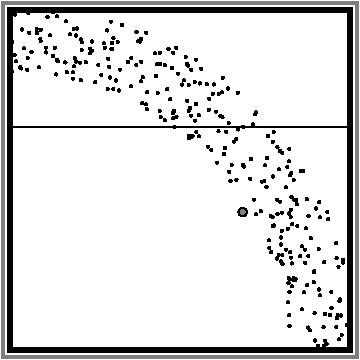
\includegraphics[width=\nnfigw]{nn-split-1} &
  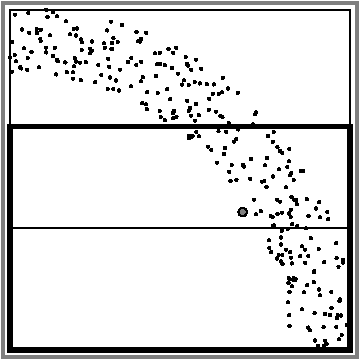
\includegraphics[width=\nnfigw]{nn-split-2} &
  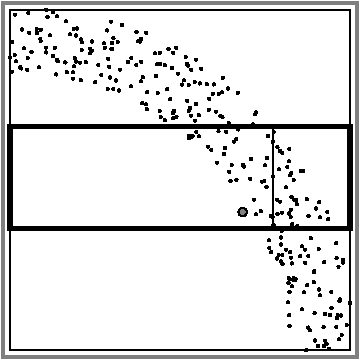
\includegraphics[width=\nnfigw]{nn-split-3} \\
      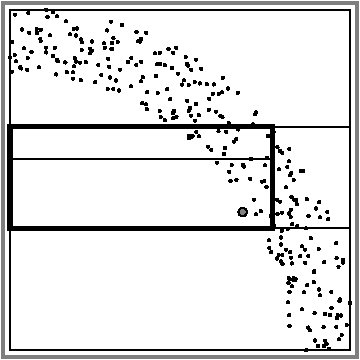
\includegraphics[width=\nnfigw]{nn-split-4} &
  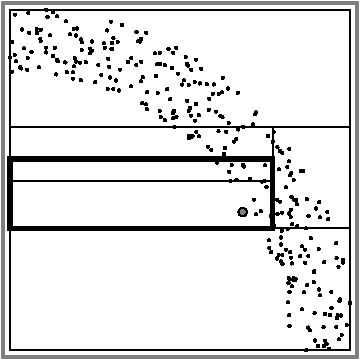
\includegraphics[width=\nnfigw]{nn-split-5} &
  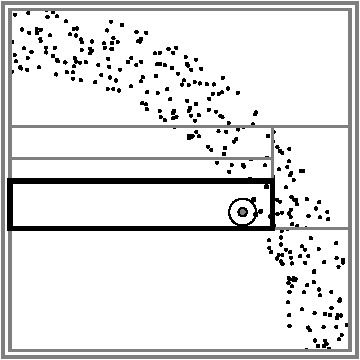
\includegraphics[width=\nnfigw]{nn-split-6}
  \end{tabular}
  \end{center}
  \caption{Nearest-neighbour search.  \captionpart{Top:} With bounding boxes.
  \captionpart{Bottom:} With splitting planes.
    The node currently being examined is
    shown in bold.  Nodes that are queued to be examined are shown with thin black
	borders.  Pruned nodes are shown with thin gray borders.  In this example,
  the first leaf node explored contains the nearest neighbour which is close enough that
   all the queued nodes can be pruned.}
  \label{fig:nn}
\end{figure}

%\clearpage

\subsection{Approximations}

\Kdtrees are applicable to approximate as well as exact algorithms.
A prominent example is the \emph{Best Bin First} (BBF) algorithm used by many
SIFT-based vision systems \cite{beis1997}.  BBF is essentially \kdtree
nearest-neighbour search where the tree traversal is ordered by a priority queue.
By terminating the search after exploring some fixed number of leaf nodes,
an approximate nearest neighbour is produced quickly.

There is an elegant solution to approximate kernel density estimation
which looks similar to the nearest-neighbour algorithm.  It refines
upper and lower bounds on the kernel density with a series of
\mindist and
\maxdist calculations.  The bounds start loose and tighten as the tree is
traversed.  The algorithm terminates when the interval is small
enough.


%%%%%%%%%%%%%%%%%%%%%%%%%%%%%%%%%%%%%%%%%%%%%%%%%%%%%%%%%%%%%%%%%%%%%%%%%%%%%%%%
\section{Efficient Implementation Tricks}
\label{sec:impl}

We consider the common case in which the \kdtree is built from a
static data set and then queried millions of times.  Although there
are some applications in which the data set must be updated online, a
number of opportunities arise when points are not added or removed
after the \kdtree is built.


This section presents a series of optimization ``tricks'' taken from
the battle-hardened \kdtree implementation at the heart of \an.
These tricks yield an order of magnitude speed increase and vastly
reduce the memory required compared to the alternatives available.


In this section, the dimension of the data points is $D$, the number
of data points is $N$, and the number of nodes in the \kdtree is $M$.
All trees are binary and complete. $N$ is large relative to $D$; for
example in the authors' application $D$ is 3 or 4, and $N$ is 10 to
100 million.  For us, the maximum tree size that fits in a 32-bit
address space is an important design parameter.

Not all of these implementation ``tricks'' apply in all cases, but each one
helps.  Although most of the tricks are concerned with reducing the memory
requirements of the \kdtree, this often has the effect of increasing the
speed as well.


\trick{Store the data points as a flat array.}
\label{trick:flatarray}
Use a one-dimensional array of size $ND$, where coordinate $j$ of data
point $i$ is stored 
%\linebreak[4]
at location $iD + j$.  For example, in three dimensions
the array will contain
\[ (x_0, y_0, z_0, x_1, y_1, z_1, \ldots) .\]

It may be tempting to store the data points as an $N \times D$
two-dimensional array.  This incurs a memory overhead of $N$ pointers,
and at runtime requires a pointer dereference.  To store one million
points in 3 dimensions ($N=10^{6}, D=3$), our {\tt libkd} requires an
overhead of 4 bytes, while the existing implementations {\tt ANN} and
{\tt simkd} use over $4$ megabytes ($8$ megabytes on 64-bit) and over
$20$ megabytes ($40$ on 64-bit), respectively.

\trick{Create a complete tree.}
\label{trick:complete}
Instead of splitting nodes until each leaf node contains some maximum
number of points, fix the number of tree levels and create a complete
tree.  The huge advantage of this trick is that the number of nodes is
known in advance, which allows the next trick to be used without
wasting any memory.

There are disadvantages to this trick.  First, the number of data
points in the leaf nodes is only adjustable by factors of two.
Second, if nodes are not split at the median value, then some leaf
nodes will contain more data points than others.

\trick{Don't use pointers to connect nodes.}
\label{trick:nopointers}
Instead, put the nodes in a single array.  Use the heap indexing
strategy shown below instead of explicit pointers.
The root is node $0$.  The left child of node $i$ is node $2i + 1$,
and the right child is node $2i + 2$.
%This works because \kdtrees are binary and complete.

\nonumberparagraphs
\begin{center}
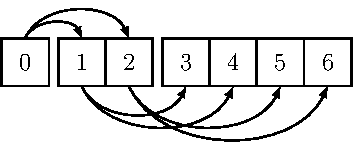
\includegraphics[width=\pointerlessfigwidth]{pointerless-fig}
\end{center}
\numberparagraphs

For a tree with $M$ nodes, this saves about $M$ pointers, and places
sibling nodes---which are likely to be accessed at the same
time---next to each other in memory.  This locality of reference
improves cache performance.


A convenient side-effect of using this trick is that the \kdtree is
position-independent: the array of nodes can be moved in memory without
changing any of the contents.  Indeed, it can be written directly to
disk in `live' form and restored at a later date.  By using the
{\tt mmap()} system call, the live on-disk representation is
immediately available for queries; the time required to read it
from disk will be amortized over the subsequent queries.  Regions of
space that are never queried may never be read from disk.


\trick{Pivot the data points while building the tree.}
\label{trick:pivot}
When building the tree, pivot the data along the splitting dimension
so that the data points owned by the child nodes are contiguous in
memory.  Represent the set of data points owned by a node as leftmost
and rightmost offsets into the data array ($L$ and $R$).  If
necessary, keep a permutation array to map from the final array
indices back to the original indices.

\nonumberparagraphs
\begin{center}
  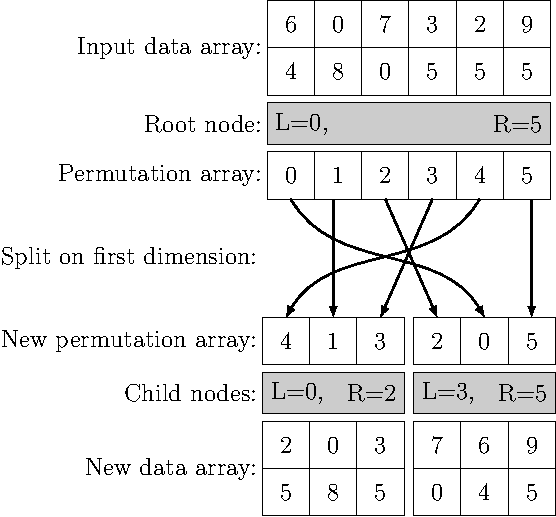
\includegraphics[width=\permutefigwidth]{permute-fig}
\end{center}
\numberparagraphs

Once this has been done, the data points owned by leaf nodes are
contiguous in memory.  In addition, leaf nodes that are nearby in
space are likely to have their data points stored nearby in memory.
This increases locality of reference and therefore performance.



\trick{Don't use {\tt C++} virtual functions.}
\label{trick:nocpp}
It may be tempting to define a class hierarchy with an abstract base
class {\tt Node} and classes {\tt InternalNode} and {\tt LeafNode}
which inherit from it (as in \secref{sec:datastruct}).  Compilers
implement this by adding a {\tt vtable} pointer to each {\tt
InternalNode} and {\tt LeafNode} object.  This enlarges each node by
the size of a pointer.  This wastes 32 (or 64) bits of memory per
node, since the node type is completely determined by its position in
the tree.  Using the node layout shown above, node $i$ is a leaf if $i
\ge M/2 - 1$ (where $M$ is the total number of nodes).  Using
inheritance also incurs an indirect function call for each virtual
function, which itself costs time and prevents the compiler from
performing inlining optimizations.




\trick{Consider discarding the permutation array.}
\label{trick:noperm}

Apply the permutation array to auxiliary data to make the \kdtree's
data order the canonical order.
For example, you might have a set of data points where each point has
a class label such as ``cat'' or ``dog''.  After creating a \kdtree
from the data points, the points are permuted so that the $i$th data
point no longer corresponds to label $i$.  However, if you apply the
inverse of the \kdtree's permutation array to the labels, they will
again correspond.  You can then discard the \kdtree's permutation
array.  This eliminates a level of indirection and a significant
amount of memory ($N$ integers).

\nonumberparagraphs
\begin{center}
  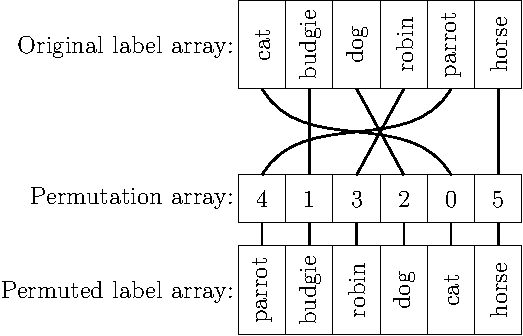
\includegraphics[width=\applypermfigwidth]{apply-perm-fig}
\end{center}
\numberparagraphs


% This is frequently the case when the index of the data serves as a
% label.  Consider a set of data points where each point has a class label
% such as ``cat'' or ``dog'' associated with it.  After creating a \kdtree
%from the data points, they will be permuted so that index $i$ in the array
%of data points no longer corresponds to index $i$ in the array of labels.
%The \kdtree's permutation array can be used to map the \kdtree's ordering
%back to the original ordering.  Alternatively, you can apply the inverse
%permutation to the array of labels.  This eliminates a level of indirection
%and a significant amount of memory from the tree.


\trick{Store only the rightmost offset of points owned by a node.}
\label{trick:ronly}

The $L$ and $R$ offsets describe the range of data points owned by a
node.  Within a level of the \kdtree, the $L$ offset of a node is
simply one greater than the $R$ offset of the node just to the left,
or zero if there is no node to the left.  Since the $L$ value can be
trivially computed from the $R$ value, there is no need to store both.
This saves $M$ integers.


\nonumberparagraphs
\begin{center}
  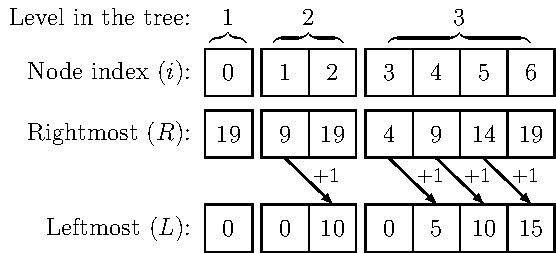
\includegraphics[width=\ronlyfigwidth]{r-only-fig}
\end{center}
\numberparagraphs

\trick{Don't store the $R$ offsets of internal nodes.}
Only leaf nodes need to store the $R$ offsets.
The leftmost data point $L$ of a non-leaf node is just the $L$ value of its
leftmost leaf.  Similarly, the rightmost data point $R$ of a non-leaf node is
$R$ of its rightmost leaf.  Try saying that ten times fast!
This saves $M/2$ integers.

%The savings are approximately $1/2\cdot${\tt sizeof(offset)}.


\trick{With median splits, don't store the $R$ offsets.}
\label{trick:noR}
Compute them instead.  If the \kdtree is built by splitting at the
median value (the common case), then the number of data points owned
by each node in the tree is a function of the total number of data
points, independent of the values of the data points.  Computing the
offsets costs $\mathcal{O}(\log M)$\footnote{There {\em may} be an
$\mathcal{O}(1)$ algorithm, though the authors haven't found it.} if
exact median splits are used and a fixed rounding direction is chosen
(\ie, the right subtree gets the extra data point when the number of
data points is odd).  However, by choosing the rounding direction
carefully---by moving the splitting position by one place---the data
points can be distributed so that the computation is $\mathcal{O}(1)$.



\trick{Consider transposing the data structures.}
\label{trick:transpose}
Instead of creating an array of {\tt node} structures, pull the
node contents directly into the {\tt kdtree} structure, creating a
separate array for each element.

\nonumberparagraphs
\begin{center}
    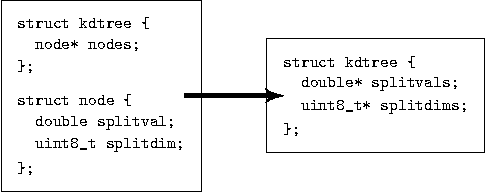
\includegraphics[width=\transposefigwidth]{transpose-fig}
\end{center}
\numberparagraphs

When a compiler encounters a structure such as {\tt node} above,
it pads the structure so that its total size is a multiple of the size of
the largest element.  For {\tt node}, the structure will be padded to 16
bytes, even though only 9 bytes are used.  It is possible to force the
compiler to pack the structure tightly, but this results in unaligned memory
accesses (many of the {\tt double} values will not start on a multiple of eight
bytes), which incurs significant overhead.


The advantage of transposing the data structures is that the memory required
can be minimized without destroying the structure alignment.  The disadvantage
is a loss of locality of reference: typically the members of a structure are
accessed at the same time, and transposing them results in the members being
dispersed in memory.

%\trick{Consider converting the data points to a smaller type.}
\trick{Consider using a smaller data type.}
\label{trick:smalltypes}
For most applications, using {\tt double} values to represent points
in $\left[0,1\right]$ is not an effective use of bits.  Consider
transforming the data to a smaller integer representation.  If the
data points live in a small bounded space, then converting {\tt
double} values to 32-bit integers saves a factor of two of space with
very little loss of precision.  Converting to 16- or 8-bit integers
saves more memory but the effect of introducing this approximation
should be considered in the context of the problem at hand.


The boundary between the \kdtree software library and the application
is an ideal place to do this transformation: the application need not
know that the \kdtree library represents the data points in a smaller
format.  The \kdtree library converts query values into the smaller
format on the way into the library, and converts results back to the
original format on the way out.  The only user-visible change should
be that the data points occupy much less memory, queries are faster,
and there may be small approximation errors.


\trick{Consider bit-packing the splitting value and dimension.}
\label{trick:packbits}
Since \kdtrees are only suitable for low-dimensional data, the
splitting dimension only requires a few bits.  Instead of storing it
in a separate array, store it in the bottom few bits of the splitting
value.  For example, with four-dimensional data points, the splitting
dimension can be stored in the bottom two bits of a 16-bit integer,
leaving 14 bits to store the splitting position.

\nonumberparagraphs
\begin{center}
  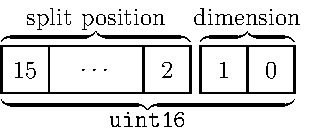
\includegraphics[width=\bitpackfigwidth]{bitpack-fig}
\end{center}
\numberparagraphs

In general, this trick conflicts with trick of not storing the $R$
offsets (\secref{trick:noR}), since that trick requires precise
control over the splitting plane location, while this trick involves
sacrificing some precision to save space.  For some data point sets,
this conflict may not arise, and both tricks may be used
simultaneously.


\trick{Consider throwing away the data.}
If your data points are associated with some other information (such
as labels), and your application can tolerate some false positive
results, consider the tradeoffs of discarding the data and keeping the
\kdtree.  By using the other tricks in this section, the memory
requirements of a \kdtree can be reduced to a small fraction of the
size of the data points themselves.  In some applications, the benefit
of being able to search more data points might outweigh the cost of
not being able to say exactly where the data points were.

Given $N$ data points, we can build a \kdtree with $N-1$ total
splitting plane nodes.  Each node contains a splitting value and
possibly the splitting dimension: it is at most slightly larger than a
single data value.  The entire tree requires about $1/D$ as much
memory as the data points themselves.

The \kdtree search algorithms then produce bounded approximations.
For nearest-neighbour search, the algorithm can produce the index of the
data point that lives in the same box as the query point, an upper bound
on the distance to that point, and a lower bound to the distance to the
true nearest neighbour.  It is also possible to produce a small list of
points that is guaranteed to contain the nearest neighbour.



\section{Speed Comparison}
\label{sec:speed}

This section gives empirical evidence that the tricks presented above
can yield significant improvements.  We compare our implementation,
{\tt libkd}, with two previously released \kdtree implementations:
{\tt ANN} \cite{arya1998} and {\tt simkd} ({\tt Simple \kdtrees})
\cite{simkd}.  We used these packages `out of the box', using the default compiler settings
and choices about how to build the \kdtree.

We chose a very simple benchmark test: the data points are 5 million
samples drawn uniformly from the unit cube ($N=5 \times 10^6, D=3$).
The number of points owned by a leaf node was set to $14$ for {\tt
ANN} and {\tt simkd} in order to make the number of nodes in the three
implementations approximately equal.  The query points are one million
samples from the same distribution.  We tested the one-nearest
neighbour algorithm.  We would have preferred to use larger $N$, since
this is the regime in which our \an project operates, but the other
libraries were not able to build such large trees.  We present results
for a 32-bit machine%
\footnote{Intel Xeon (SL72G) at 3.06 GHz with 4 GB of RAM.}
and a 64-bit machine%
\footnote{AMD Opteron 8220 SE at 2.8 GHz with 32 GB of RAM.}
to show how the memory requirements differ.

\begin{table}
\begin{center}
\newcommand{\ftt}[1]{{\tt #1}}
\newcommand{\minitab}[2][l]{\begin{tabular}{#1}#2\end{tabular}}
\newcommand{\sg}[1]{{\small #1}}
\newcommand{\libkdmem}[3]{\multicolumn{2}{c|}{%
    \makebox[\widthof{\sg{120 +}}][r]{\sg{#1 +}} %
    \makebox[\widthof{\sg{52}}][r]{\sg{#2}} = %
    \makebox[\widthof{172}][r]{#3}}}
\newcommand{\compmem}[3]{\multicolumn{1}{c|}{%
    \makebox[\widthof{\sg{120 +}}][r]{\sg{#1 +}} %
    \makebox[\widthof{\sg{250}}][r]{\sg{#2}} = %
    \makebox[\widthof{370}][r]{#3}}}
\begin{tabular}{|l|D{.}{}{3.0}@{\hspace{5pt}}D{.}{}{3.0}|r@{\hspace{5pt}}r|}
\hline
\multirow{3}{*}{\minitab[c]{{\bf Implementation}}} &
%
\multicolumn{2}{c|}{{\bf Speed}} &
\multicolumn{2}{c|}{{\bf Memory}} \\
&
\multicolumn{2}{c|}{(k q/sec)} &
\multicolumn{2}{c|}{data + tree = total (Mbytes)} \\
& \multicolumn{1}{c}{32-bit}
& \multicolumn{1}{c|}{64-bit}
& \multicolumn{1}{c}{32-bit}
& \multicolumn{1}{c|}{64-bit} \\
\hline
\ftt{simkd} &          47. &  39. & \compmem{120}{250}{370} & \compmem{120}{366}{486} \\
\ftt{ANN}   &          71. &  90. & \compmem{120}{67}{187} & \compmem{120}{101}{221} \\
\hline
\ftt{libkd-d-box}   & 127. & 144. & \libkdmem{120}{52}{172} \\
\ftt{libkd-d-split} & 231. & 284. & \libkdmem{120}{6}{126} \\
\ftt{libkd-d-noR}   & 239. & 293. & \libkdmem{120}{5}{125} \\
\ftt{libkd-i-split} & 242. & 311. & \libkdmem{ 60}{4}{64} \\
\ftt{libkd-i-noR}   & 240. & 326. & \libkdmem{ 60}{3}{63} \\
\ftt{libkd-s-split} & 328. & 386. & \libkdmem{ 30}{3}{33} \\
\ftt{libkd-s-noR}   & 307. & 396. & \libkdmem{ 30}{2}{32} \\
\hline
\end{tabular}
\end{center}
\caption{Benchmark results.
Speed is measured in thousands of queries per second (k q/sec), memory
in megabytes.  The memory values include the memory required to store
the data points themselves, which is $120$ MB when {\tt double}s are
used.  For the {\tt libkd} entries, {\tt d} indicates that the data
points are stored as {\tt double}, {\tt i} indicates 32-bit integers,
and {\tt s} indicates 16-bit integers (using
trick \ref{trick:smalltypes}).  {\tt box} means that bounding-boxes
are created; otherwise splitting-planes are used.  The {\tt noR}
entries indicate that the we avoid storing the offset arrays
(trick \ref{trick:noR}).  We have also assumed that trick
\ref{trick:noperm} is applicable, so the permutation arrays are not stored.}
\label{table:results}
\end{table}

\begin{figure}
    \begin{center}
    \begin{tabular}{@{}c@{}c@{}}
    \kdbarmemfig & \kdbarspeedfig
    \end{tabular}
    \end{center}
    \caption{Benchmark results.
        %
\captionpart{Left:} Memory requirements of the various
implementations.  The {\tt simkd} and {\tt ANN} methods use different
amounts of memory on 32- and 64-bit machines because the size
of pointers is larger in 64-bit machines, and these methods
use many pointers.  {\tt libkd} uses no pointers internally so
uses the same amount of memory on 32-bit and 64-bit machines.
The memory usage of {\tt libkd} is significantly smaller than
the competing implementations.  When using 32-bit or 16-bit
integers ({\tt i} and {\tt s} variants, respectively) to store
the data, rather than {\tt doubles}, the memory requirements
are reduced even further, though at the expense of some
approximation error.
%
\captionpart{Right:} Speed (in thousands of queries per second) of the
various implementations.  {\tt libkd} is always faster than the
competition.  The splitting-plane variant is significantly faster than
the bounding-box variant.  The {\tt noR} trick seems to help on the
64-bit machine but have little effect on the 32-bit machine.  Note
that the 64-bit CPU is an AMD while the 32-bit CPU is an Intel, so
these differences are likely due to the many differences in the chips
rather than the word size \latin{per se}.  Given these differences,
practitioners are urged to perform benchmarks on their own hardware
and their own data.\label{fig:results}}
\end{figure}

Table \ref{table:results} and \figref{fig:results} show our results.
Our implementation, {\tt libkd}, always takes less memory and produces
faster results.  The memory requirements of {\tt ANN} and {\tt simkd}
increase when using a 64-bit machine, while {\tt libkd} stays fixed
because we use no extraneous pointers.  Note that the data points
themselves require $120$ MB of space, so the memory overhead of a {\tt
libkd} tree is only a few percent, compared to $50$ to $300$ percent
for {\tt ANN} and {\tt simkd}.

In this test, splitting planes are much faster than bounding boxes.
Using trick \ref{trick:noR} to avoid storing the offset arrays both
reduces the memory required and slightly increases the speed.  Using
trick \ref{trick:smalltypes} to use smaller data types (32- and 16-bit
integers) reduces the memory footprint by a factor of two or four,
with a corresponding increase in speed.  It also incurs some
approximation error.  In this test, we found that when using 32-bit
integers, we still always produced the correct nearest neighbour, and
the absolute error in the distance estimates was never more than
$10^{-9}$.  When using 16-bit integers, we produced the correct
nearest neighbour 99.5\% of the time, and the absolute distance error
was less than $10^{-4}$.

% actual approximation errors; 4x10^{-10} and 8x10^{-5}.

In summary, these results show that, on this benchmark, by using the
tricks presented {\tt libkd} is three times faster and incurs
one-fifteenth the memory overhead compared to the closest competitor.
While benchmarks are not listed among the three canonical types of
lies (``lies, damned lies, and statistics''), we urge practitioners to
test these implementations on their own data.  Our testing and
benchmarking software is available for download.


% cluster59:
% (?) http://processorfinder.intel.com/Details.aspx?sSpec=SLABS

% cluster23:
%    2 * Intel(R) Xeon(TM) CPU 3.06GHz
%    S-spec SL72G
%    http://processorfinder.intel.com/details.aspx?sSpec=SL72G
%    4 GB RAM
%    32-bit
%    libkd: -O3
%           -DNDEBUG
%           -march=pentium4
%           -fomit-frame-pointer
%           -fno-math-errno
%           -fno-trapping-math
%           -fno-signaling-nans
%           -ffinite-math-only
%    ann: -O3
%    simkd: -O2

% testB.in
% 5M points in 3D
% 120 MB data
% ann, simkd: bucket size 14
% libkd: bucket size 10

% simkd:
%  516,748 leaves
%  370 MB including data

% ann:
%  516,748 leaves
%  187 MB including data

% libkd:
%  524,288 leaves
%  172 MB ddd/bbox
%  126 MB ddd/split
%  125 MB ddd/nolr
%   64 MB duu/split
%   63 MB duu/splitdim/linearlr
%   33 MB dss/split
%   32 MB dss/splitdim/linearlr

% speed: q/sec:
%   47  simkd
%   71  ann
%
%  127  ddd/bbox
%  231  ddd/split
% (203) ddd/nolr
%  239  ddd/linearlr
%
%  242  duu/split
% (233) duu/splitdim
% (205) duu/splitdim/nolr
%  240  duu/splitdim/linearlr
%
%  328  dss/split
% (303) dss/splitdim
% (255) dss/splitdim/nolr
%  307  dss/splitdim/linearlr



% cluster27:
%    4 * AMD Opteron(tm) Processor 8220 SE
%    32 GB RAM
%    64-bit
%    libkd: -O3
%           -DNDEBUG
%           -march=k8 -m64
%           -fomit-frame-pointer
%           -fno-signaling-nans
%           -ffinite-math-only
%           -fno-math-errno
%           -fno-trapping-math
%    ann: -O3
%    simkd: -O2

% testB.in
% 5M points in 3D
% 120 MB data
% ann, simkd: bucket size 14
% libkd: bucket size 10

% simkd:
%  516,865 leaves
%  486 MB including data

% ann:
%  516,785 leaves
%  221 MB including data

% libkd:
%  524,288 leaves
%  172 MB ddd/bbox
%  126 MB ddd/split
%  125 MB ddd/nolr
%   64 MB duu/split
%   63 MB duu/splitdim/linearlr
%   33 MB dss/split
%   32 MB dss/splitdim/linearlr

% speed: q/sec:
%   39  simkd
%   90  ann
%
%  144  ddd/bbox
%  284  ddd/split
% (260) ddd/nolr
%  293  ddd/linearlr
%
%  311  duu/split
% (314) duu/splitdim
% (287) duu/splitdim/nolr
%  326  duu/splitdim/linearlr
%
%  386  dss/split
% (378) dss/splitdim
% (341) dss/splitdim/nolr
%  396  dss/splitdim/linearlr





\section{Conclusion}

\Kdtrees are a fun and easy data structure for searching in $k$-dimensional
space. A careful implementation can be orders of magnitude faster than
a na\"ive one. Readers wishing to reap the benefits of such a careful
implementation, without building it themselves, are encouraged to
download the GPL'd {\tt libkd}. Patches are welcome!

